\documentclass{article}
\usepackage[utf8]{inputenc}
\usepackage{fancyhdr}
\usepackage{graphicx}
\usepackage{geometry}

% ---- Commands ------- %
\newcommand{\documentNumber}[1]{
    \LARGE  \textbf{ PUSS2142{#1} } \\
    \medskip
}
\newcommand{\documentVersion}[1]{
    v. {#1}

    \medskip
}
\newcommand{\documentTitle}[1]{
    \centerline{\rule{13cm}{0.4pt}}
    \bigskip \bigskip
    \LARGE \textbf{TimeMate} \\
    \bigskip
    \LARGE {#1} \\
    \bigskip \bigskip
    \centerline{\rule{13cm}{0.4pt}}
}
\newcommand{\documentGroup}[1]{
    \bigskip \bigskip
    \LARGE Group {#1} \\
    \bigskip
}
\newcommand{\documentResponsible}[1]{
    \LARGE Responsible: {#1} \\
    \medskip
}
\newcommand{\documentAuthors}[1]{
    \LARGE Authors: {#1} \\
    \medskip    
}
\newcommand{\documentDate}[1]{
    \date {#1} 
}

\graphicspath{{./images/}} % Defines a path to file images
\renewcommand{\arraystretch}{1.7}  % Vertical padding for tables


% --- Header & Footer ---- %
\pagestyle{fancy}
\lhead{\leftmark}
\rhead{}
\rfoot{\thepage}
\cfoot{}
\lfoot{}


% ------------------------------------------------ #

% ----- FILL THIS ----- %
\title {
    \documentNumber {08}
    \documentVersion {0.3}
    \documentTitle {Project Final Report}
    \documentGroup {2}
    \documentResponsible {Project Management Group}
    \documentAuthors {Project Management Group}
    \documentDate {2021-03-21}
}

\begin{document}

\maketitle
\thispagestyle{empty}

\newpage

\tableofcontents

\newpage

\section{Document History}
\begin{tabular}{ l | l | l | l }
    Version & Date & Responsible & Description \\
    \hline
    0.1 & 2021-03-17 & PG & Document created. \\
    \hline
    0.2 & 2021-03-19 & PG & Ready for informal review. \\
    \hline
    0.3 & 2021-03-21 & PG & Fixed typos and grammar mistakes. Document ready for hand-in. \\
\end{tabular}

\section{Terminology}
    \begin{table}[h]
        \centering
        \begin{tabular}{| l | l |}
            \hline
                DG & Developer Group \\
            \hline
                PG & Project management Group \\
            \hline
                SG & System management Group \\
            \hline
                TG & Test Group \\
            \hline
                SDDD & Software Detailed Design Document \\
            \hline 
                SDP & Software Development Plan \\
            \hline
                SRS & Software Requirements Specification \\
            \hline
                SSD & System Specification Document \\
            \hline
                STLDD & Software Top Level Design Document \\
            \hline
                SVVR & Software Verification and Validation Report \\
            \hline
                SVVI & Software Verification and Validation Instruction \\
            \hline
                SVVS & Software Verification and Validation Specification \\
            \hline
        \end{tabular}
        \caption{Terminology}
        \label{Terminology}
    \end{table}

\section{Referenced Documents \label{refs}}
    \begin{itemize}
        \item Software Development Plan, v. 1.1, Doc. number: PUSS214200.
        \item \label{PH} Project Instruction (Projekthandledningen).
    \end{itemize}

\newpage

\section{Executive Summary}
    This report summarises the work done by project group 2 in the course \emph{ETSF20, Programvaruutveckling för stora projekt}. The project took place during January, February and March of 2021. It involved 21 students and 3 faculty members at Lund University. The aim of this project was to give students practical experience of working in a large group with the aim to produce a time reporting system. Whilst the software was the end product, this report mainly focuses on the lessons learned during the course of the project. The group delivered a product that met the requirements and did so within the allotted time frame.
    \\ \\
    This report is structured as follows: Section \ref{overview} gives an overview of the
    project. Section \ref{analysis} presents an analysis of the results and aims to answer questions regarding taken decisions and challenges that were faced. Section \ref{tips} gives six tips for future project groups, and at last, section \ref{conclusion} gives a conclusion
    that contains reflections from the entire project group.

\section{Project Overview \label{overview}}
    This section aims to give an overview of the project and is structured as follows:
    Section \ref{phase1} to \ref{phase4} describes the work process for each phase as well as how they went. Figures are included which displays the reported time from each member of the group. Sections \ref{reported_time} to \ref{system_locally} describe other aspects of the project that were present throughout.
    
    \subsection{Phase 1. Week 3-5 \label{phase1}}
        PG started planning and gathering the group during week 2 to prepare for phase 1.
        The first phase started with an overwhelming amount of information that everyone
        had to digest. At the same time, big decisions had to be taken such as creating groups,
        creating a timeplan and certain design choices.
        \\ \\
        Writing the SDP, SRS and SVVS, which would lay the ground work for the next couple of months, went well. However the first informal
        review failed to catch most of the critical errors, which led to the formal reviewer not approving the documents for baseline and
        requiring us to hand in the documents for approval after adjustments.
        \\ \\
        After reworking the documents and our review process, we held a second informal review. This time, the remarks were
        significantly more useful but the meeting structure did not support the ensuing discussions. The need for a second informal review and
        some scheduling issues for the formal review cost us three days. During the transition into phase 2 we took what we had learned and
        made adjustments to our review methods.

        \begin{figure}[!htb]
            \minipage{0.32\textwidth}
              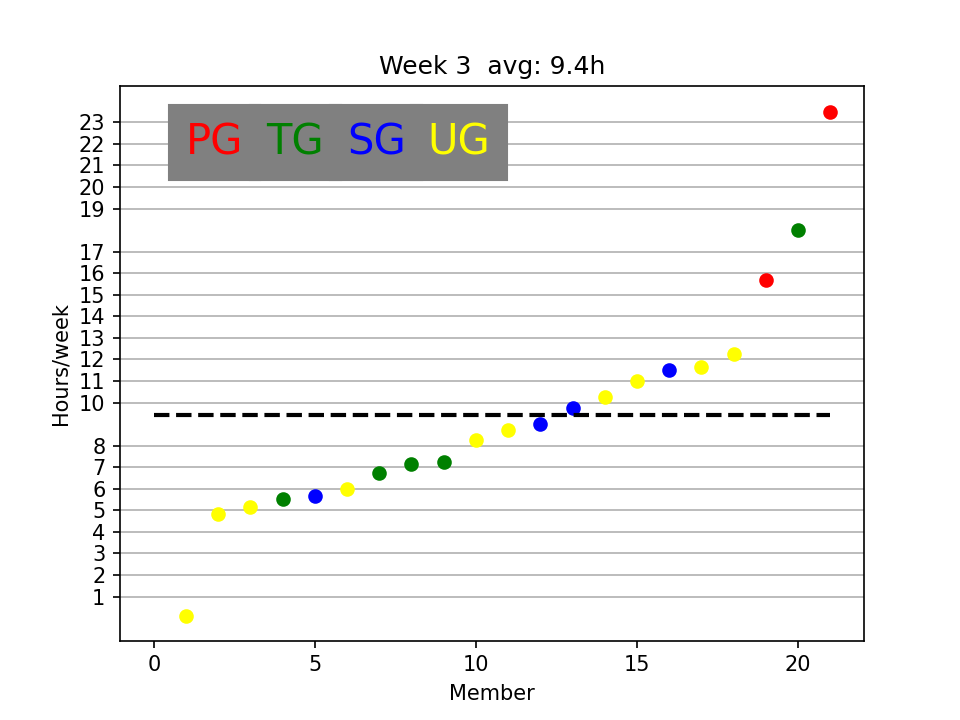
\includegraphics[width=\linewidth]{images/week_3.png}
              \caption{Worked hours week 3.}\label{fig:week3}
            \endminipage\hfill
            \minipage{0.32\textwidth}
              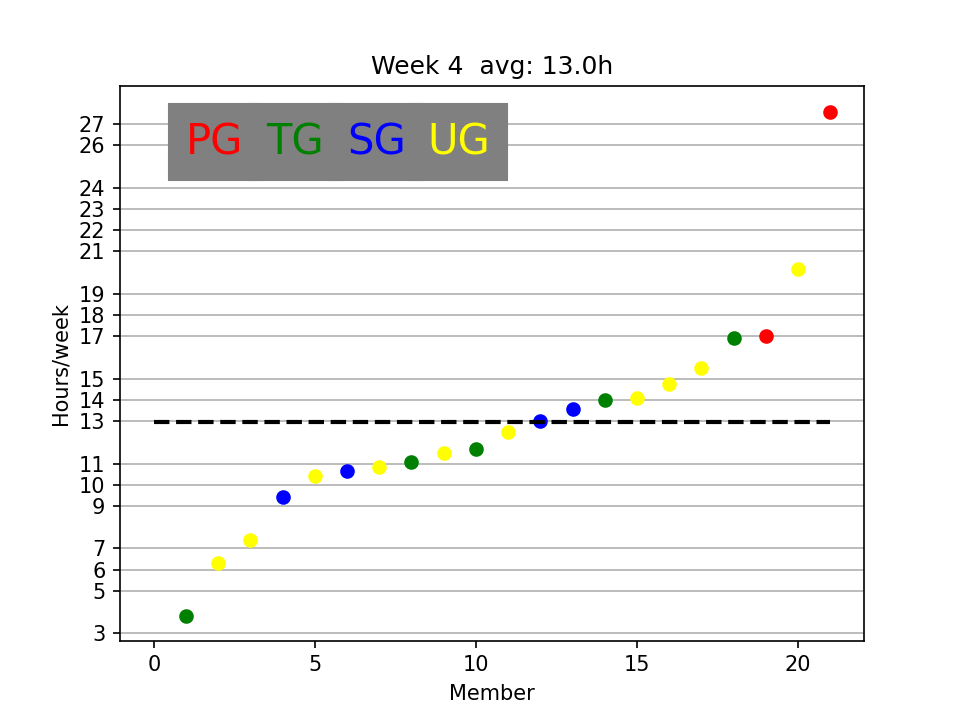
\includegraphics[width=\linewidth]{images/week_4.png}
              \caption{Worked hours week 4.}\label{fig:week4}
            \endminipage\hfill
            \minipage{0.32\textwidth}%
              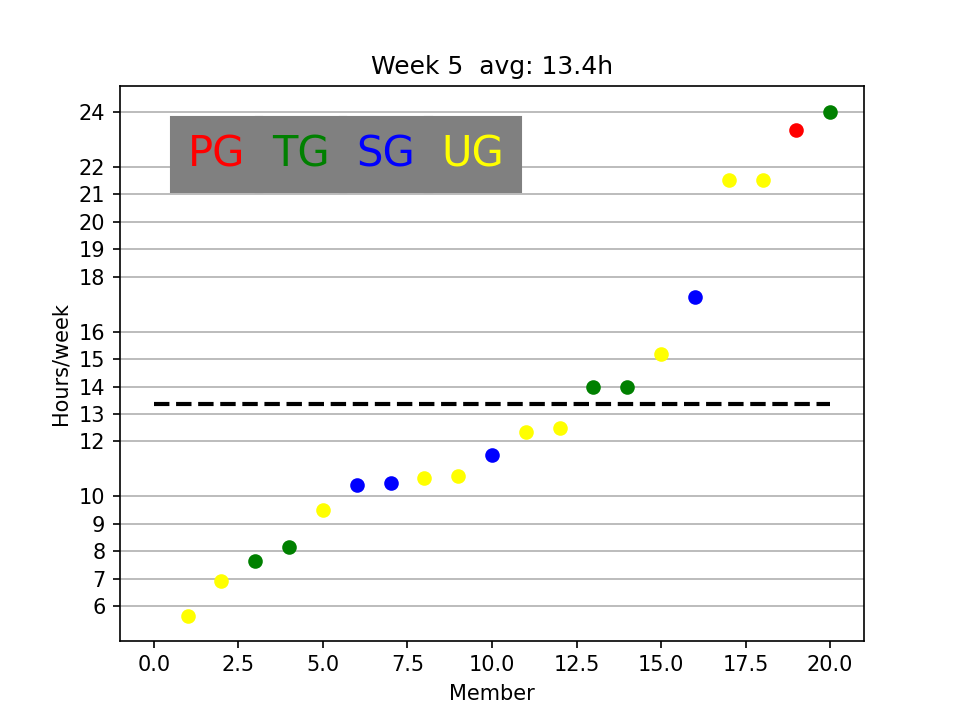
\includegraphics[width=\linewidth]{images/week_5.png}
              \caption{Worked hours week 5.}\label{fig:week5}
            \endminipage
        \end{figure}

    \subsection{Phase 2. Week 6-7 \label{phase2}}
        Due to the delay at the end of phase 1, the second phase was compressed to stay on schedule. 
        There was a slight panic at the beginning of the phase as the document deadline was closer than some group 
        members had anticipated. This was solved by clear and concrete scheduling and effective work distributions within the development group. They scheduled an extra work shift and dedicated 3 members to do graphics for
        the STLDD, which helped pipeline the writing process. DG had spent some time during phase 1 preparing for 
        this document, which gave them a running start when it was time to write.
        \\ \\
        The writing of SVVI went straightforward as TG was very focused throughout the phase. This focus remained
        during the entire project and the test group never had any big issues.
        \\ \\
        The formal review went well, the reviewer only had a few remarks, but left it up to the group to correct them and put the documents in baseline.
        Several members from TG and DG were tasked with this, whilst the rest of the group
        started with development and testing for phase 3. Getting a head start in the next phase whilst others finished up the current
        phase became a common strategy, even if it went against the strict rules outlined in the waterfall method.
        
        \begin{figure}[!htb]
            \minipage{0.16\textwidth}
            \endminipage\hfill
            \minipage{0.32\textwidth}
              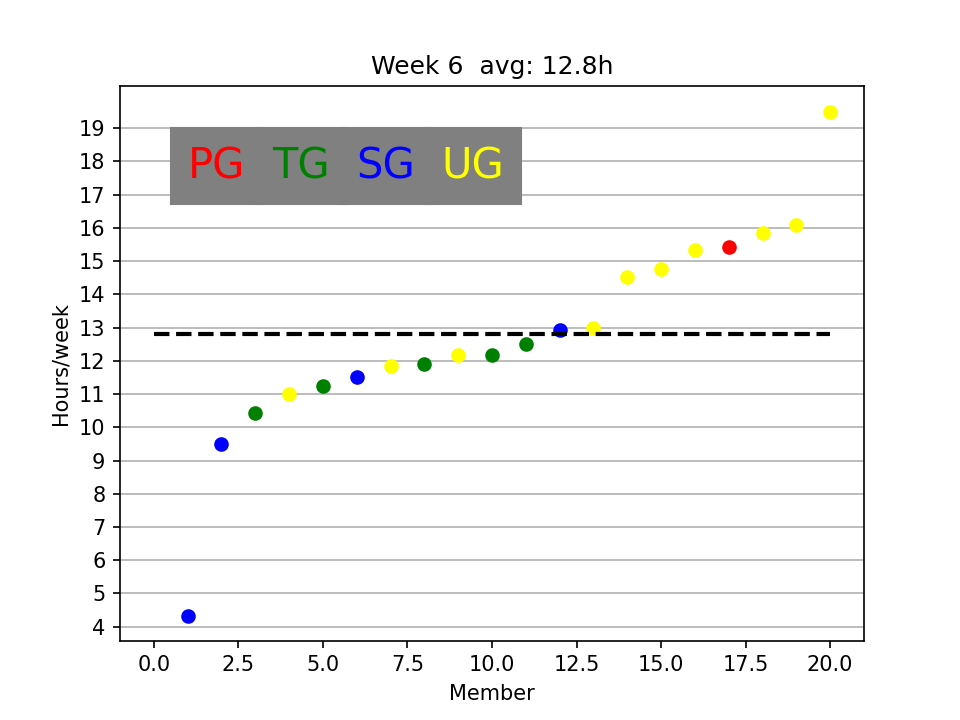
\includegraphics[width=\linewidth]{images/week_6.png}
              \caption{Worked hours week 6.}\label{fig:week6}
            \endminipage\hfill
            \minipage{0.32\textwidth}
              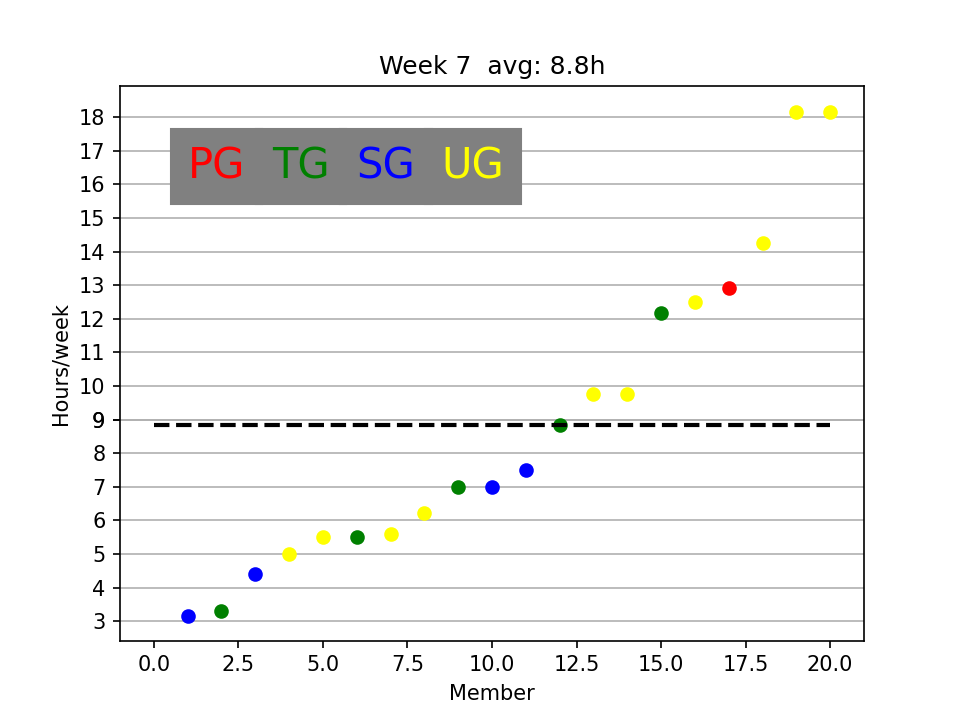
\includegraphics[width=\linewidth]{images/week_7.png}
              \caption{Worked hours week 7.}\label{fig:week7}
            \endminipage\hfill
            \minipage{0.16\textwidth}
            \endminipage\hfill
        \end{figure}
        
    \subsection{Phase 3. Week 8-9 \label{phase3}}
        Phase 3 \emph{unofficially} started on time, but \emph{officially} we were 3 days behind schedule, due to
        the formal review result in Phase 2. This meant that the group had roughly a week to develop the software
        before the first informal review. This caused some panic and many members did not believe that the
        deadline would be reached.
        \\ \\
        DG spent a lot of time trying to translate the contents of STLDD to code
        and ambiguities started to show regarding how the system was supposed to fit together.
        This meant that valuable time that should have been spent producing running code, was
        instead spent on understanding the STLDD as well as the SRS.
        \\ \\
        The purpose and responsibilities of SG were somewhat unclear. The initial plan was that SG
        was to aid DG, handle the communication between DG and TG and assist any of the
        groups if needed. It seemed like there were either a misunderstanding of this, or a lack of
        communication between SG and the rest, because according  to SG, no one needed help, but in
        reality, DG was quite far behind even early in phase 3.
        This lead to \emph{heroes}
        emerging, group members that put in considerably more hours than others, as seen in figure \ref{fig:week9}.
        \\ \\
        The informal review was pushed forward a day and reviewing of code
        convention and code style was ignored due to the code being unfinished. Instead, only
        functional tests and system tests were performed, all of which were successful. However, there
        were still minor discrepancies between the system and the SRS, as well as plenty of
        undocumented and ugly code. 
        \\ \\
        The second informal review was pushed from Friday to the Tuesday of week 10, which was enough
        for the group fix the corrections. However, after this review, further fixes were required,
        such as deleting unused variables and adding javadoc comments. Further corrections were made and on Friday week 10 the SDDD reached baseline.
        
        \begin{figure}[!htb]
            \minipage{0.16\textwidth}
            \endminipage\hfill
            \minipage{0.32\textwidth}
              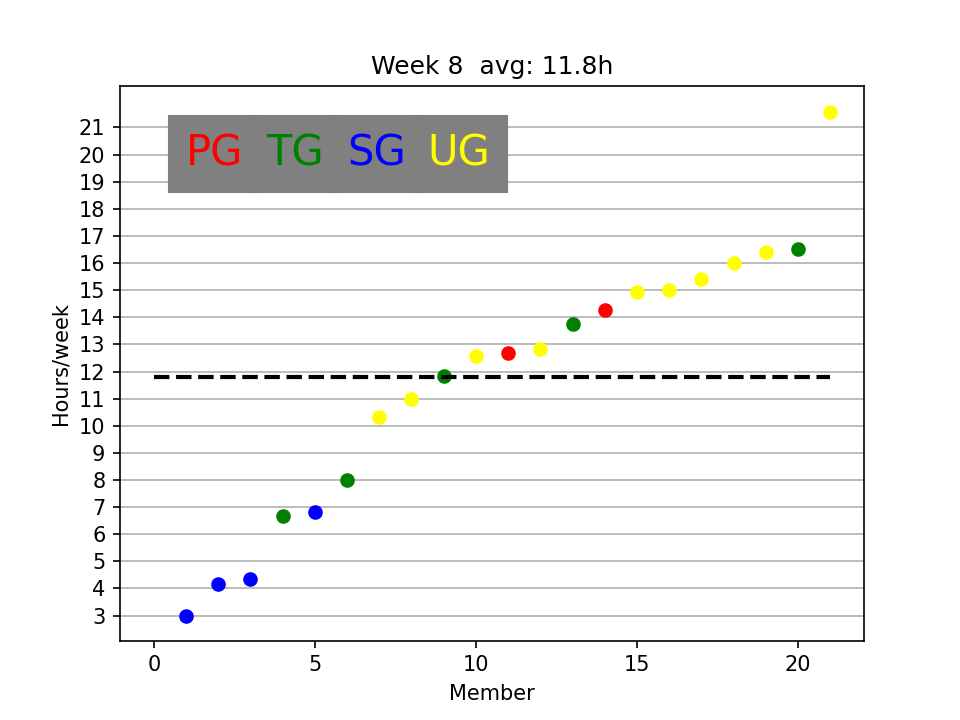
\includegraphics[width=\linewidth]{images/week_8.png}
              \caption{Worked hours week 8.}\label{fig:week8}
            \endminipage\hfill
            \minipage{0.32\textwidth}
              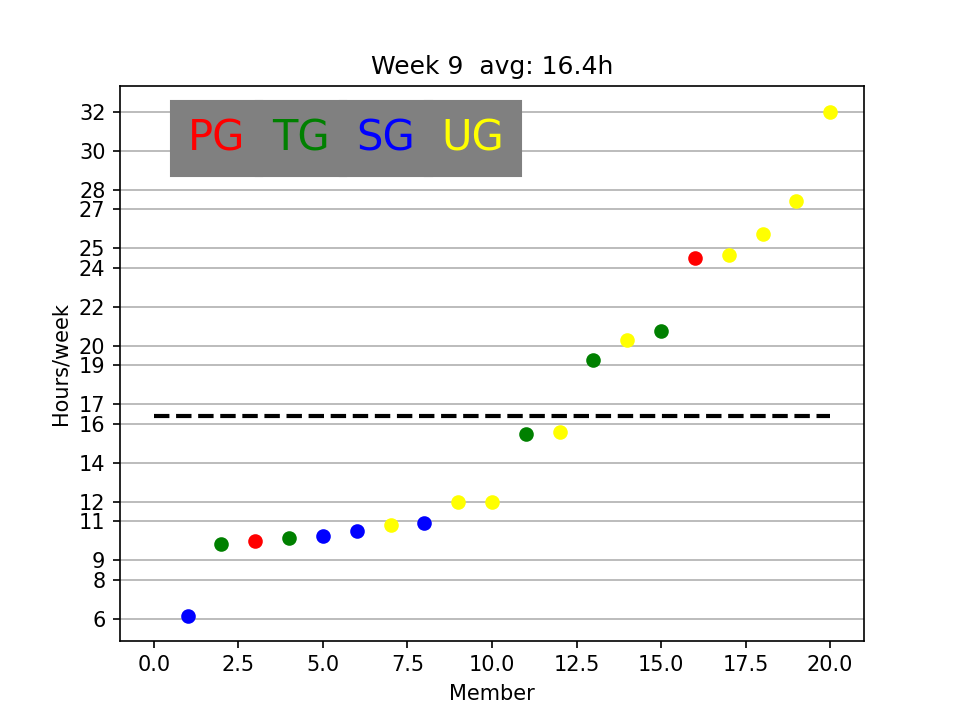
\includegraphics[width=\linewidth]{images/week_9.png}
              \caption{Worked hours week 9.}\label{fig:week9}
            \endminipage\hfill
            \minipage{0.16\textwidth}
            \endminipage\hfill
        \end{figure}
        
        
    \subsection{Phase 4. Week 10-11 \label{phase4}}
        Once the SDDD had reached baseline the project was put on hold as the group
        studied for the upcoming exams (week 11 was exam week). However, during the time that
        that DG spent finishing the software, the other groups started working on documents for phase 4.
        Two out of the three documents were almost done by the time phase 4 \emph{officially} started.
        \\ \\
        The last project group meeting was on the Tuesday of week 11 and the last informal review took
        took place the following Friday. Figure \ref{fig:week10} clearly shows that the project was \emph{not}
        a priority during this week. Because this report was written during week 11, its time report graph is not included.
        \begin{figure}[!htb]
            \centering
            \minipage{.32\textwidth}
              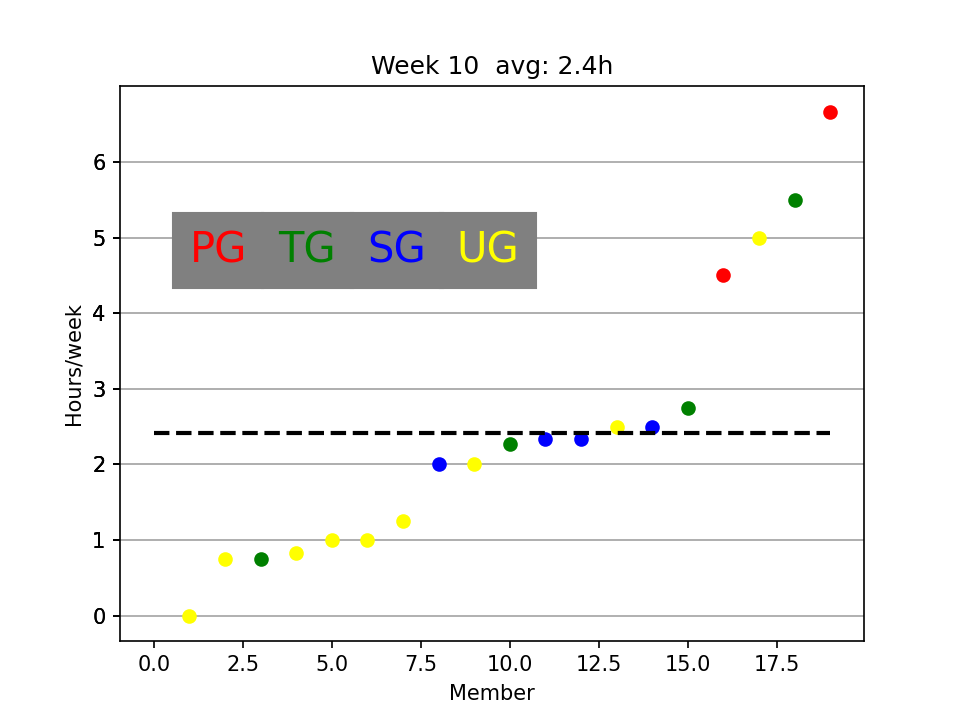
\includegraphics[width=\linewidth]{images/week_10.png}
              \caption{Worked hours week 10.}\label{fig:week10}
            \endminipage\hfill
        \end{figure}

    \subsection{Reported Time \label{reported_time}}
        Figure \ref{fig:final} illustrates the average hours/week spent for each week.
        This number (9.8h/week) is very close to the expected value stated in SDP which was 10
        hours per week. However, even though the \emph{average} hours worked during the project came out to be 
        almost exactly what was expected, it is clear from figure \ref{fig:week3} to \ref{fig:week10}
        that the hours were \emph{not} evenly distributed. Heroes started to emerge early
        on and while this was discussed as a potential risk early in the project, it seemed unavoidable.
        \\ \\
        After week 5, PG showed graphs from reported work time to point out the differences and 
        invited the people who had spent less time to spend more, and to the ones who spent more time,
        to spend less as well as to ask for help. What impact this had is unknown.
    
        \begin{figure}[!htb]
            \centering
            \minipage{.32\textwidth}
              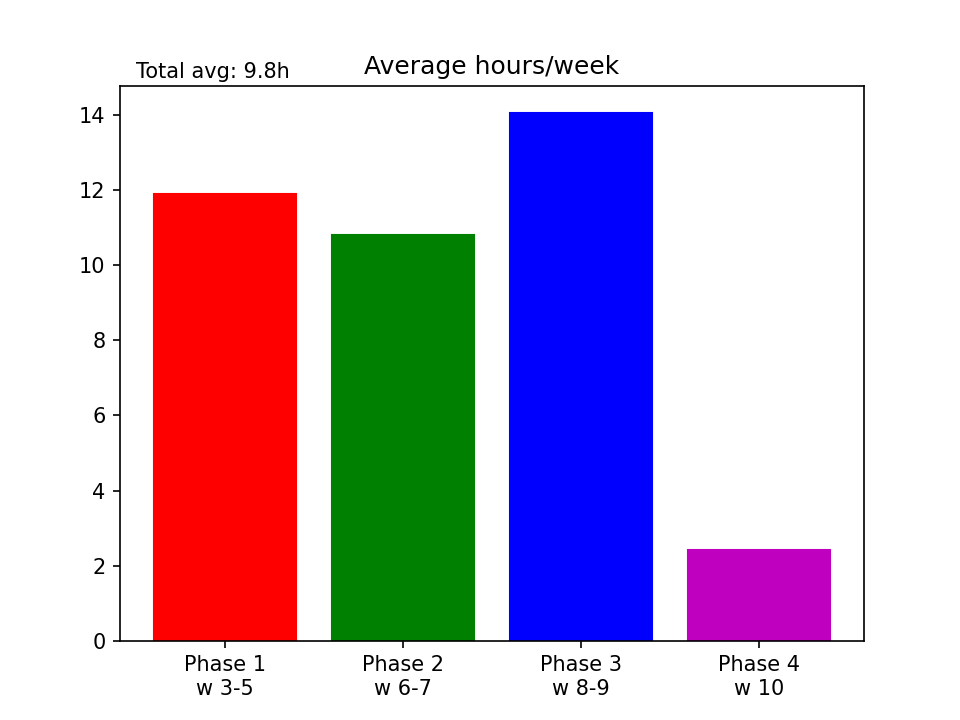
\includegraphics[width=\linewidth]{images/final.png}
              \caption{Summary of average worked hours during the project.}\label{fig:final}
            \endminipage\hfill
        \end{figure}

    \subsection{Staying on Schedule}
        As described in sections \ref{phase1} to \ref{phase4} each phase was
        delayed by a few days. Figure \ref{fig:schedule}
        illustrates the differences between the planned schedule and when
        baselines were actually reached.
        
        \begin{figure}[!htb]
            \centering
            \minipage{1\textwidth}
              \includegraphics[width=\linewidth]{images/phase_bar_graph.png}
              \caption{Graph comparing the estimated time for each phase to outcome. }\label{fig:schedule}
            \endminipage\hfill
        \end{figure}
      
      \subsection{Version Control \& Configuration Management \label{cm}}
        The decision to use git as version control was taken during phase 1
        and it worked quite well. The few issues that occurred, were small and easy to deal with.
        To educate the group, PG held a 45 minute long education of basic usage of git which was also
        recorded so that members that missed it could watch it afterwards.
        \\ \\
        While git was used to update files, E-PUSS was used to track the version numbers
        of the documents. These were recorded in the Status Reports and worked well.
        \\ \\
        One thing that differed from the initial plan of git usage was when updating
        the version of a document that had reached baseline. For this to work efficiently,
        a \emph{patch} branch was created which forked from the \emph{development} branch.
        The updated document was then put into the \emph{patch} branch which then got merged %Do you merge 'with' or 'to' a branch?
        to \emph{master}. This process took a little longer, but seemed like a solid solution that kept the \emph{master} branch up to date, and secure.
        \\ \\
        Figure \ref{fig:commits_total} and \ref{fig:commits} illustrates the commit distribution
        and commit history during the project. As of writing this report, a total of 18 out of 21 group members have committed to the GitHub repository with a total of 1,139 commits.
        
        \begin{figure}[!htb]
            \minipage{0.16\textwidth}
            \endminipage\hfill
            \minipage{0.32\textwidth}
              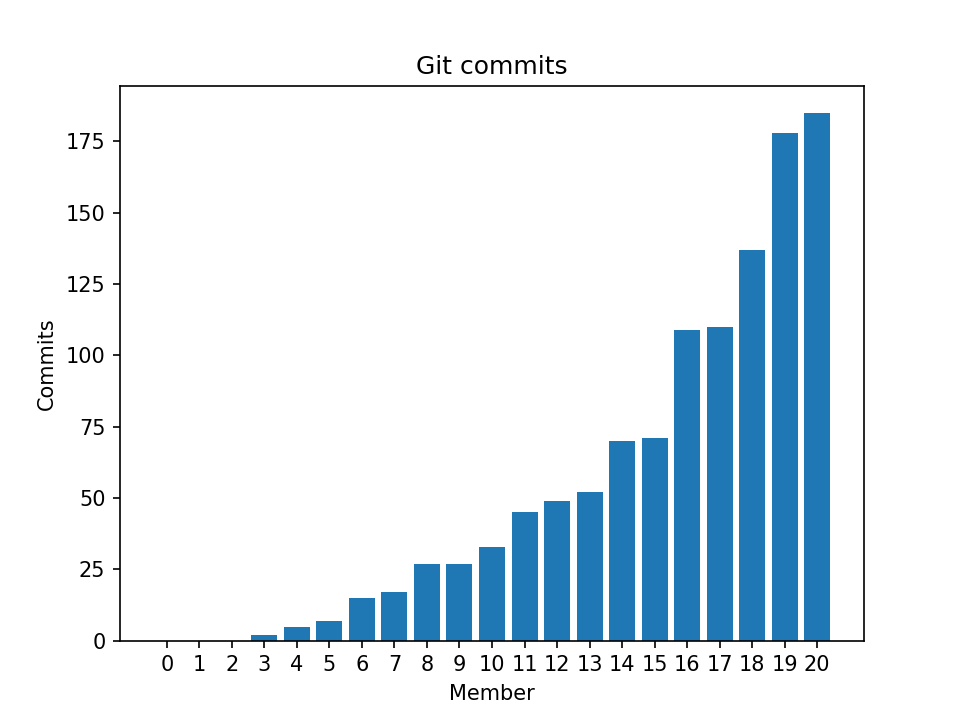
\includegraphics[width=\linewidth]{images/commits.png}
              \caption{Commit distributed throughout the group.}\label{fig:commits}
            \endminipage\hfill
            \minipage{0.32\textwidth}
              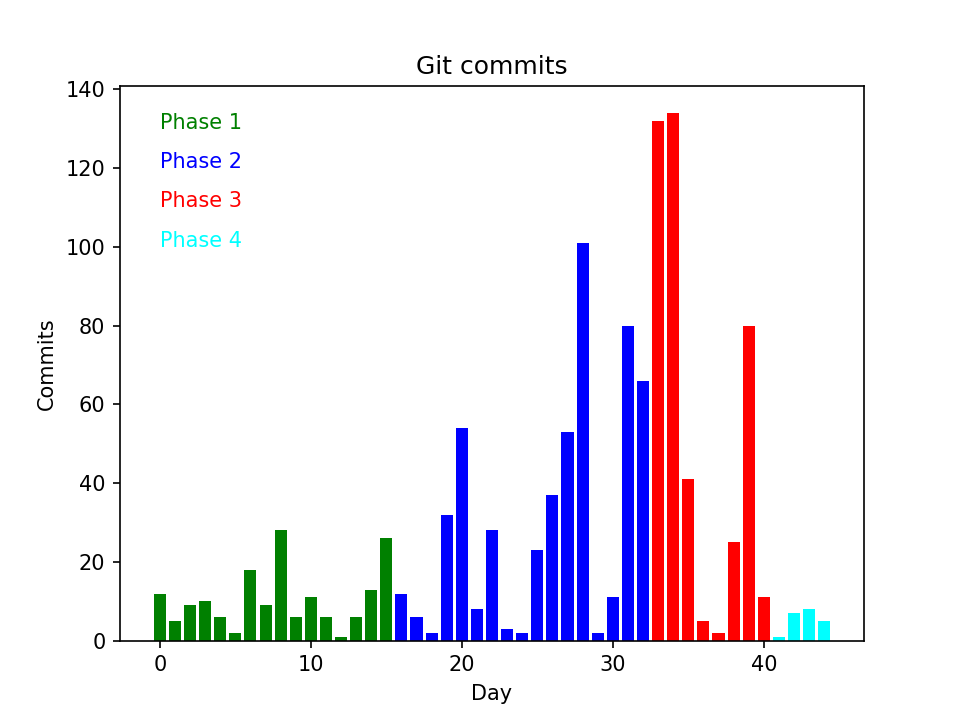
\includegraphics[width=\linewidth]{images/commits_total.png}
              \caption{Commits for each phase.}\label{fig:commits_total}
            \endminipage\hfill
            \minipage{0.16\textwidth}
            \endminipage\hfill
        \end{figure}

    \subsection{Status \& Problem reports}
        In total, 15 problem reports were filed during the project. Out of these, 5 got rejected and the remaining 10 resulted in an update of the documents which lead to an update of the status reports.
        However, some of the problem reports were logically connected and thus only resulted
        in a single update in the status reports.
        \\ \\
        As seen in figure \ref{fig:versions} most documents did not require more than one or two changes
        after baseline was reached. Documents for phase 4 are not included in the figure since none of the documents
        for the phase were in baseline during the writing of this report.
        
        \begin{figure}[!htb]
            \centering
            \minipage{.32\textwidth}
              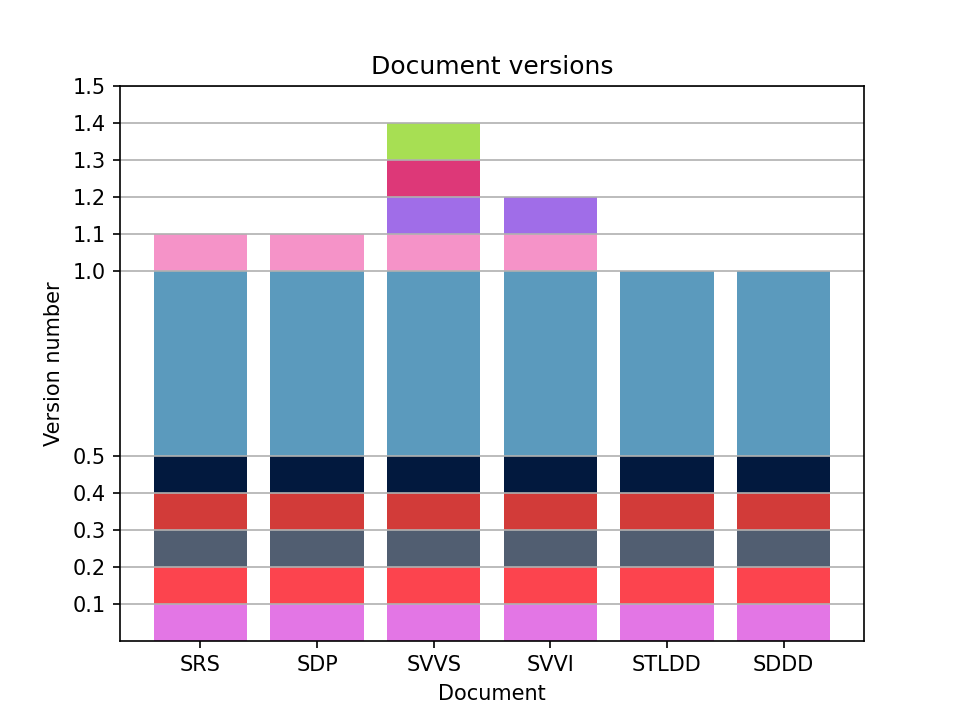
\includegraphics[width=\linewidth]{images/document_versions.png}
              \caption{Document version numbers from phase 1-3.}\label{fig:versions}
            \endminipage\hfill
        \end{figure}
        
    \subsection{Online Communication \label{communication}}
        After the first project meeting (held on Zoom) the decision to move to
        Discord was taken. For the remainder of the project Discord served as the only communication channel
        and worked flawlessly.
        \\ \\
        However, while the online communication worked very well for the most part, it resulted
        in a lack of connection between group members. For instance, even though two of
        the ground rules specified in SDP were to actively participate during meetings,
        and, as much as possible have the camera on, this did not happen.

        The majority of the time during the project group meetings was
        spent as a monologue from the president with just a few cameras on.
        When discussions occurred it was mostly the same people who participated, which resulted
        in about 15 people not saying a word during most of the meetings.
        This caused frustration among PG as it was difficult to gauge the opinion of the group.
    
    \subsection{Running the system locally \label{system_locally}}
        Getting the system to run locally caused more issues than expected and even late
        into phase 3 there were several members that could not get it to work.
        To aid people with this, a cheat sheet was created which included step by step
        instructions how to get the system running. Though it is unknown if and how
        much this helped, it seemed like reasonable solution.
        
    \subsection{Group Managers}
        Besides the project managers, we appointed a manager for each work group SG, DG and TG. The tasks of the system manager and test manager were outlined in the Project Instructions and were quite clear, but the role of development manager was not specified and thus \emph{not} clear.
        This resulted in the ambiguities regarding the responsibilities, purpose of the role. This also leads to certain tasks falling between the cracks or being
        delayed, such as splitting DG into groups, telling inner groups in DG what to do, etc.

    \subsection{Project Forms}
        Figure \ref{fig:form_0} to \ref{fig:form_4} shows the result of an anonymous form that
        was sent to each member in the group during the writing of this report. 18 out of 21 members
        replied.

        \begin{figure}[!htb]
            \minipage{0.32\textwidth}
              \includegraphics[width=\linewidth]{images/form_0.png}
              \caption{Experienced stress.}\label{fig:form_0}
            \endminipage\hfill
            \minipage{0.32\textwidth}
              \includegraphics[width=\linewidth]{images/form_1.png}
              \caption{Spent time.}\label{fig:form_1}
            \endminipage\hfill
            \minipage{0.32\textwidth}
              \includegraphics[width=\linewidth]{images/form_2.png}
              \caption{Enjoyable project.}\label{fig:form_2}
            \endminipage\hfill
        \end{figure}

        \begin{figure}[!htb]
            \minipage{0.16\textwidth}
            \endminipage\hfill
            \minipage{0.32\textwidth}
              \includegraphics[width=\linewidth]{images/form_3.png}
              \caption{Communication.}\label{fig:form_3}
            \endminipage\hfill
            \minipage{0.32\textwidth}
              \includegraphics[width=\linewidth]{images/form_4.png}
              \caption{Knowing what to do.}\label{fig:form_4}
            \endminipage\hfill
            \minipage{0.16\textwidth}
            \endminipage\hfill
        \end{figure}


\section{Analysis \label{analysis}}
    This section describes our perception of how the project went and how it lined up with our expectations.
    This section follows the same structure as the Project Overview.

    \subsection{Phase 1. Week 3-5} 
        During the first informal review, the bulk of the remarks were made up of grammar and spelling errors, rather
        than flaws in the  content. This was an issue since the documents being reviewed clearly needed more work, as demonstrated
        by them not being approved for baseline by the formal reviewer. To correct this, we introduced a guiding document that was
        supposed to aid reviewers. The idea of this document was to be a reference for all future reviews, and 
        thus cointained information about reviewing code that would have to be filtered out when 
        reviewing a docuement and vice versa. The complexity of the document was suspected to be an issue but it did help to some extent, because the next batch of reviewers remarks were more useful.
        \\ \\
        The influx of useful remarks exposed another flaw in our review process. The initial plan for the meeting was
        that each reviewer presented their remarks, which would then be either accepted or discussed further. 
        The reference document had failed to mention how a reviewer should organize their
        remarks, which, along with the superfluous meeting structure, led to poorly structured presentations and discussions that were hard to follow.
        \\ \\
        To ensure the quality of future reviews we discarded the reference document and took a simpler
        approach that borrowed heavily from the format of the formal reviews. Reviewers got a review 
        guide that was specific to the item being reviewed and all remarks were put into a
        table. The remarks were sent to the authors of the document before the meeting. During the review meeting,
        only remarks that warranted discussion were mentioned. This procedure was kept during the rest of the project and it worked very well.
        \\ \\
        We also aimed at improving the work distribution and staying on schedule. The following measures were taken:
        \begin{itemize}
            \item Increase the scheduled work shifts from 1 to 2 per week.
            \item Have PG engage more with the groups, instead of relying on group leaders to act as a 
            bridge between management and other members. 
            \item Redistribute tasks from PG to SG and TG. 
        \end{itemize}
        
    \subsection{Phase 2. Week 6-7}
        Group members were getting more comfortable with their roles and
        tools which became visible since everything worked very well. In total, phase 2 documents probably had an equal amount of issues as the phase 1 documents but
        most of these issues were found during the informal review and could be corrected before the formal review.
        As a result we could make some final changes and put the documents in baseline ourselves, saving us a day or two.
        
    \subsection{Phase 3. Week 8-9 \label{analys_phase3}}
        As explained in section \ref{phase3} this phase became quite stressful and 
        was a week late to reach baseline. The reason behind the stress and delay was
        probably a combination of the following:
        \begin{itemize}
            \item Important and time-consuming activities in other courses.
            \item Poor understanding of how the system was actually supposed to be work and
                    be put together.
            \item Lack of communication between the subgroups of DG which resulted in
                    extra work, such as different variable names between frontend/backend.
            \item SG feeling unsure of what to do, which meant that they were not utilized.
                    Figure \ref{fig:week8} and \ref{fig:week9} clearly illustrates this as
                    SG only spent an average of 7 hours while DG spent 17 hours on average.
            \item Uncertainties in SRS, which resulted in ambiguities regarding system requirements.
                    For instance, certain design choices were either not specified or not
                    specific enough, which resulted in DG having to improvise.
            \item Lack of knowledge and experience with the technologies, which meant that valuable time
                    was spent doing research on how certain technologies or frameworks work (like jsp, tomcat etc). This should have been done earlier in the project so that phase 3 could be entirely about implementing the STLDD instead of googling.
            \item The waterfall method is not suited for a project when the group has zero to little experience with the technology. Because of this, we believe that an agile development method would be more suitable for this project.
        \end{itemize}
        \noindent
        Section \ref{analyse_schedule} and \ref{analyse_system} presents possible solutions to prevent some of issues mentioned.
    
    \subsection{Phase 4. Week 10-11}
        This phase was very straightforward and by the time phase 3 reached baseline, the larger parts of SSD and SVVR were already finished.
        During this phase, the tasks of the different roles are also more defined.
        Though we must note that as of the writing of this document phase 4 is not over, so issues may still arise.

    \subsection{Reported Time}
        While the group did agree early to avoid heroes, they did occur anyways.
        Unfortunately we believe that this is unavoidable and a natural result of working in a big group of people. We motivate this rather cynical statement with the fact that people take school more or less serious and have different goals and ambitions. If a group with three students where student A and B
        aims to learn as much as possible and are ready to work 10 hours a week, while student C only wants to
        pass the course and is not ready to put more than 5 hours a week, person A and B will work harder than person C.
        \\ \\
        This was not unexpected and in fact, something that PG pointed out very early on. On several occasions
        members were encouraged to talk about their goals and ambitions so they would get an understanding
        of what to expected from each other. Whether this had an impact or not is unknown, but we felt that there was not much more to do.
    
    \subsection{Staying on Schedule \label{analyse_schedule}}
        The schedule was kept with minor deviations, but we did underestimate the time it would take
        to reach a baseline for most of the documents. We believed that baseline would be reached straight
        after formal review, without any marks. This turned out to be quite naive since none of the formal reviews resulted in baseline without \emph{any} adjustments required.
        \\ \\
        Several members felt that more time should have been spent during phase 3 and
        this was in fact the initial plan. However, after a discussion, the group \emph{did} take
        the decision to schedule two weeks for phase 3. Whilst more time during phase 3
        obviously would have made it less stressful, one can argue that the reason it was stressful
        was not because of lack of time, but rather because of poor communication between the groups,
        poor preparation and the rest of the possible reasons mentioned in section \ref{analys_phase3}. Also,
        if more time would be spent on phase 3, the time has to come from somewhere, for instance phase 2, but then there
        would be less time to do the planning. Thus we propose the following improvements if we were do the project again:
        \begin{itemize}
            \item PG should be more strict from the beginning and be \emph{very} clear regarding what each group
                    should do and what their responsibilities are. 
            \item DG should choose their groups during the first week, giving them sufficient time to prepare.
        \end{itemize}

    \subsection{Version Control \& Configuration Management}
        As explained in section \ref{cm} there were 3 members that did not make a single
        commit to the project repository. While the cause of this is unknown, we consider
        one of the following explanations:
        \begin{enumerate}
            \item They do not know how to use git.
            \item They have worked in groups and thus not needed to commit anything themselves.
            \item They have not participated in the project.
        \end{enumerate}
        As we will not investigate this any further we do believe that it would have been
        better if every member was forced to do several pushes to the repository as soon
        as the decision to use git was taken. This would reduce the chances that people
        do not know how to use the tool and thus eliminate option 1. 
    
    \subsection{Status \& Problem reports}
        Even though the UI of E-PUSS is a bit dated, the functionality worked
        pretty well for creating problem reports and handling status reports.
        Even though git has support for both of these, the amount of work and time to ensure
        that everyone gets the education required to use it did not seem worth it and thus
        we believe that it was the right decision to use E-PUSS.
    
    \subsection{Online Communication}
        The biggest benefit of online communication was that it was very easy and quick to
        contact people and to share files, join different rooms etc. It was also easier for
        people to participate during meetings since no traveling was required.
        However, as described in section \ref{communication} the lack of participation and active cameras
        had a negative impact on the communication.
    
    \subsection{Running the system locally \label{analyse_system}}
        To reduce problems to get the system running locally, 
        we conclude in the following possible solutions:
        \begin{enumerate}
            \item Set a deadline for everyone to get the system running locally. 
                    A list could be used so that each member can sign when they have
                    the system running as well as a help list if they need guidance.
                    This would force people to get the system running and PG and SG
                    would notice who had not.
            \item While out of our hands, the lab work in this course should have been held earlier.
        \end{enumerate}
        
    \subsection{Group Managers}
        We believe that the issue with the developer manager role could have been prevented by carefully specifying the responsibilities of the
        role in the beginning of the project and having more discussions with the person who had the role.
        Another option would be to \emph{not} have a development manager
        and instead give the responsibilities to SG. This could also result in the role and purpose of 
        SG becoming more clear, which as discussed in section \ref{analys_phase3} was a problem during phase 3.

    \subsection{Project Forms}
        As seen in figure \ref{fig:form_0} to \ref{fig:form_4} the results indicate
        that even though the project was stressful, most people enjoyed it and believed that
        the communication generally worked well. However there are still room for improvements
        and in the following section, we aim to share some tips to make the graphs look even prettier
        for future groups.


\section{Six tips for future project groups \label{tips}}

    To help future project groups we have compiled a list of six tips that we would like to share.
    They come as a result of the project and the lessons we have learned.
    
    \subsection{Tip 1}
        In the beginning, ensure that you spend enough time to fully understand the purpose and the
        responsibility for each role. Spending more time on this early on will be useful as the project
        goes on as it will help to ensure that everyone knows what to do, and what their responsibilities are. It is also crucial
        to convey this information to the groups.
        
    \subsection{Tip 2}
        Since this semester has four courses running in parallel, it could be a nice idea
        to schedule times for the group to not only work on the project, but also to study
        for other courses. This could improve the team building and communication within the
        group and ensure that people do not fall behind in other courses. As the pressure of other
        courses contributed to the stress felt by the group, this would also have a positive effect on group morale.
    
    \subsection{Tip 3}
        Ensure that you know what you want to get out of the informal reviews. The following
        questions can be used:
        \begin{enumerate}
            \item \emph{Who} is reviewing?
            \item \emph{What} should the reviewer look for?
            \item \emph{Where} should the comments/notes from the reviewer be, and in what format?
        \end{enumerate}
        Also remember that the informal reviews are meant to catch errors and \emph{improve}
        the documents. It is pointless to have a review if everyone just agrees and finds nothing. 
        We believe it is better to be \emph{too} hard than too gentle.
        
    \subsection{Tip 4}
        Just like any other programming project, development time is very hard to estimate. 
        The third phase was by far the most stressful due to optimistic planning and delays caused by earlier phases. 
        When making a schedule for a future project, it would be wise to give development as much time as possible and 
        take into account that things do not always work out of the box.
        
    \subsection{Tip 5}
        Use each phase as a learning experience, be open to altering your procedures based on feedback from the group, \emph{even if} it requires making changes to baselined documents.
        
    \subsection{Tip 6}
        Feedback does not come on its own. Setting up a system for constant feedback from the group could aid in identifying bottle necks and in turn, improving efficiency.
    
\section{Conclusion \label{conclusion}}
    An important thing to consider is the external stress factor that other courses, and separate
    modules of this course, introduced. It has been a shared sentiment within the group that the 
    work load during this semester has been overwhelming. Several group members have had issues 
    balancing school work, some even putting other courses on hold. Whilst it is expected of a 
    student who studies at full pace to put 40 hours/week into their school work, the reality 
    of the situation is that most do not. The the sudden jump in time required had a big impact 
    on the stress level felt by the group. Despite this, the group came together and worked hard to get results.
    \\ \\
    TimeMate was delivered on time and all requirements were met. By this metric it would be
    fair to say that the project went well. There are multiple lessons to take away from this project, all of which are very important.
    As preparation, as well as during, the writing of this report the group discussed the project. The perception within the group is
    that the project was fun and very valuable from an academic standpoint. So in conclusion, the members of project group 2 are proud of
    their collective effort and consider this project to have been a rather stressful, but an equally valuable experience.
    
\newpage
\section{Acknowledgements}
    Thank you to Christine Lindholm for you guidance and patience. \\ \\
    Thank you to Emelie Engström for making our documents legible. \\ \\
    Thank you to Anders Bruce for your technical expertise. \\ \\
    Lastly, a big thank you to every member in group 2:
    \begin{itemize}
        \item Victor Krook (PG)
        \item Assar Orpana (PG)
        \item David Vilppu (SG Leader)
        \item Ramtin Mosavi (SG)
        \item Filip Sjövall (SG)
        \item Mustafa Elomeiri (SG)
        \item Oscar Johansson (DG Leader)
        \item Alexandra Galonja (DG)
        \item Anna Bergvall (DG)
        \item Annelie Sinander (DG)
        \item Hjalmar Janson (DG)
        \item Sebastian Forslund (DG)
        \item Abd Salam (DG)
        \item Alaa Wahbah (DG)
        \item Alexander Olofsson (DG)
        \item Johan Wulf (DG)
        \item Alexander Möhle (TG Leader)
        \item Lazar Trpeski (TG)
        \item Max Palmgren (TG)
        \item Malte Wallander (TG)
        \item Anas Abu Al-Soud (TG)
    \end{itemize}

\end{document}
